% Created by tikzDevice version 0.12.6 on 2024-03-28 21:55:23
% !TEX encoding = UTF-8 Unicode
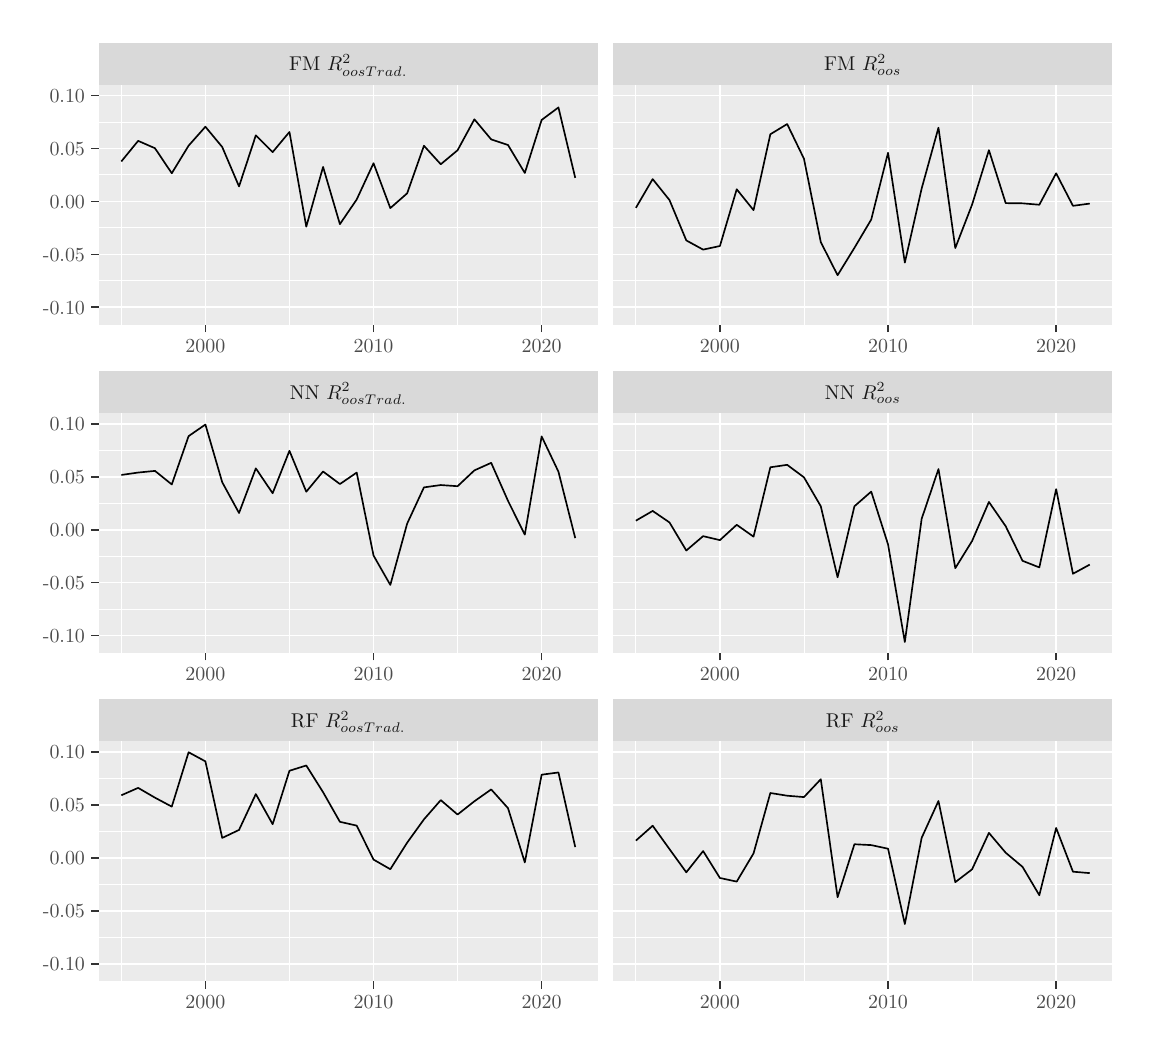
\begin{tikzpicture}[x=1pt,y=1pt]
\definecolor{fillColor}{RGB}{255,255,255}
\path[use as bounding box,fill=fillColor,fill opacity=0.00] (0,0) rectangle (397.48,361.35);
\begin{scope}
\path[clip] (  0.00,  0.00) rectangle (397.48,361.35);
\definecolor{drawColor}{RGB}{255,255,255}
\definecolor{fillColor}{RGB}{255,255,255}

\path[draw=drawColor,line width= 0.6pt,line join=round,line cap=round,fill=fillColor] (  0.00,  0.00) rectangle (397.48,361.35);
\end{scope}
\begin{scope}
\path[clip] ( 25.65,254.04) rectangle (206.07,340.69);
\definecolor{fillColor}{gray}{0.92}

\path[fill=fillColor] ( 25.65,254.04) rectangle (206.07,340.69);
\definecolor{drawColor}{RGB}{255,255,255}

\path[draw=drawColor,line width= 0.3pt,line join=round] ( 25.65,269.86) --
	(206.07,269.86);

\path[draw=drawColor,line width= 0.3pt,line join=round] ( 25.65,289.00) --
	(206.07,289.00);

\path[draw=drawColor,line width= 0.3pt,line join=round] ( 25.65,308.14) --
	(206.07,308.14);

\path[draw=drawColor,line width= 0.3pt,line join=round] ( 25.65,327.27) --
	(206.07,327.27);

\path[draw=drawColor,line width= 0.3pt,line join=round] ( 33.85,254.04) --
	( 33.85,340.69);

\path[draw=drawColor,line width= 0.3pt,line join=round] ( 94.59,254.04) --
	( 94.59,340.69);

\path[draw=drawColor,line width= 0.3pt,line join=round] (155.34,254.04) --
	(155.34,340.69);

\path[draw=drawColor,line width= 0.6pt,line join=round] ( 25.65,260.30) --
	(206.07,260.30);

\path[draw=drawColor,line width= 0.6pt,line join=round] ( 25.65,279.43) --
	(206.07,279.43);

\path[draw=drawColor,line width= 0.6pt,line join=round] ( 25.65,298.57) --
	(206.07,298.57);

\path[draw=drawColor,line width= 0.6pt,line join=round] ( 25.65,317.70) --
	(206.07,317.70);

\path[draw=drawColor,line width= 0.6pt,line join=round] ( 25.65,336.84) --
	(206.07,336.84);

\path[draw=drawColor,line width= 0.6pt,line join=round] ( 64.22,254.04) --
	( 64.22,340.69);

\path[draw=drawColor,line width= 0.6pt,line join=round] (124.97,254.04) --
	(124.97,340.69);

\path[draw=drawColor,line width= 0.6pt,line join=round] (185.72,254.04) --
	(185.72,340.69);
\definecolor{drawColor}{RGB}{0,0,0}

\path[draw=drawColor,line width= 0.6pt,line join=round] ( 33.85,313.01) --
	( 39.92,320.45) --
	( 46.00,317.78) --
	( 52.07,308.74) --
	( 58.15,318.71) --
	( 64.22,325.55) --
	( 70.30,318.22) --
	( 76.37,303.98) --
	( 82.44,322.44) --
	( 88.52,316.38) --
	( 94.59,323.66) --
	(100.67,289.44) --
	(106.74,311.03) --
	(112.82,290.35) --
	(118.89,299.26) --
	(124.97,312.36) --
	(131.04,296.15) --
	(137.12,301.48) --
	(143.19,318.67) --
	(149.27,311.99) --
	(155.34,317.05) --
	(161.42,328.23) --
	(167.49,320.97) --
	(173.57,318.94) --
	(179.64,308.84) --
	(185.72,328.01) --
	(191.79,332.52) --
	(197.86,307.08);
\end{scope}
\begin{scope}
\path[clip] ( 25.65,135.43) rectangle (206.07,222.07);
\definecolor{fillColor}{gray}{0.92}

\path[fill=fillColor] ( 25.65,135.43) rectangle (206.07,222.07);
\definecolor{drawColor}{RGB}{255,255,255}

\path[draw=drawColor,line width= 0.3pt,line join=round] ( 25.65,151.25) --
	(206.07,151.25);

\path[draw=drawColor,line width= 0.3pt,line join=round] ( 25.65,170.38) --
	(206.07,170.38);

\path[draw=drawColor,line width= 0.3pt,line join=round] ( 25.65,189.52) --
	(206.07,189.52);

\path[draw=drawColor,line width= 0.3pt,line join=round] ( 25.65,208.65) --
	(206.07,208.65);

\path[draw=drawColor,line width= 0.3pt,line join=round] ( 33.85,135.43) --
	( 33.85,222.07);

\path[draw=drawColor,line width= 0.3pt,line join=round] ( 94.59,135.43) --
	( 94.59,222.07);

\path[draw=drawColor,line width= 0.3pt,line join=round] (155.34,135.43) --
	(155.34,222.07);

\path[draw=drawColor,line width= 0.6pt,line join=round] ( 25.65,141.68) --
	(206.07,141.68);

\path[draw=drawColor,line width= 0.6pt,line join=round] ( 25.65,160.81) --
	(206.07,160.81);

\path[draw=drawColor,line width= 0.6pt,line join=round] ( 25.65,179.95) --
	(206.07,179.95);

\path[draw=drawColor,line width= 0.6pt,line join=round] ( 25.65,199.09) --
	(206.07,199.09);

\path[draw=drawColor,line width= 0.6pt,line join=round] ( 25.65,218.22) --
	(206.07,218.22);

\path[draw=drawColor,line width= 0.6pt,line join=round] ( 64.22,135.43) --
	( 64.22,222.07);

\path[draw=drawColor,line width= 0.6pt,line join=round] (124.97,135.43) --
	(124.97,222.07);

\path[draw=drawColor,line width= 0.6pt,line join=round] (185.72,135.43) --
	(185.72,222.07);
\definecolor{drawColor}{RGB}{0,0,0}

\path[draw=drawColor,line width= 0.6pt,line join=round] ( 33.85,199.72) --
	( 39.92,200.59) --
	( 46.00,201.19) --
	( 52.07,196.29) --
	( 58.15,213.75) --
	( 64.22,217.94) --
	( 70.30,197.08) --
	( 76.37,185.98) --
	( 82.44,202.10) --
	( 88.52,193.11) --
	( 94.59,208.45) --
	(100.67,193.67) --
	(106.74,200.98) --
	(112.82,196.43) --
	(118.89,200.58) --
	(124.97,170.61) --
	(131.04,159.98) --
	(137.12,182.13) --
	(143.19,195.23) --
	(149.27,196.08) --
	(155.34,195.65) --
	(161.42,201.38) --
	(167.49,204.10) --
	(173.57,190.35) --
	(179.64,178.17) --
	(185.72,213.65) --
	(191.79,200.90) --
	(197.86,176.91);
\end{scope}
\begin{scope}
\path[clip] ( 25.65, 16.81) rectangle (206.07,103.46);
\definecolor{fillColor}{gray}{0.92}

\path[fill=fillColor] ( 25.65, 16.81) rectangle (206.07,103.46);
\definecolor{drawColor}{RGB}{255,255,255}

\path[draw=drawColor,line width= 0.3pt,line join=round] ( 25.65, 32.63) --
	(206.07, 32.63);

\path[draw=drawColor,line width= 0.3pt,line join=round] ( 25.65, 51.77) --
	(206.07, 51.77);

\path[draw=drawColor,line width= 0.3pt,line join=round] ( 25.65, 70.90) --
	(206.07, 70.90);

\path[draw=drawColor,line width= 0.3pt,line join=round] ( 25.65, 90.04) --
	(206.07, 90.04);

\path[draw=drawColor,line width= 0.3pt,line join=round] ( 33.85, 16.81) --
	( 33.85,103.46);

\path[draw=drawColor,line width= 0.3pt,line join=round] ( 94.59, 16.81) --
	( 94.59,103.46);

\path[draw=drawColor,line width= 0.3pt,line join=round] (155.34, 16.81) --
	(155.34,103.46);

\path[draw=drawColor,line width= 0.6pt,line join=round] ( 25.65, 23.06) --
	(206.07, 23.06);

\path[draw=drawColor,line width= 0.6pt,line join=round] ( 25.65, 42.20) --
	(206.07, 42.20);

\path[draw=drawColor,line width= 0.6pt,line join=round] ( 25.65, 61.33) --
	(206.07, 61.33);

\path[draw=drawColor,line width= 0.6pt,line join=round] ( 25.65, 80.47) --
	(206.07, 80.47);

\path[draw=drawColor,line width= 0.6pt,line join=round] ( 25.65, 99.61) --
	(206.07, 99.61);

\path[draw=drawColor,line width= 0.6pt,line join=round] ( 64.22, 16.81) --
	( 64.22,103.46);

\path[draw=drawColor,line width= 0.6pt,line join=round] (124.97, 16.81) --
	(124.97,103.46);

\path[draw=drawColor,line width= 0.6pt,line join=round] (185.72, 16.81) --
	(185.72,103.46);
\definecolor{drawColor}{RGB}{0,0,0}

\path[draw=drawColor,line width= 0.6pt,line join=round] ( 33.85, 83.98) --
	( 39.92, 86.65) --
	( 46.00, 83.11) --
	( 52.07, 79.87) --
	( 58.15, 99.52) --
	( 64.22, 96.23) --
	( 70.30, 68.56) --
	( 76.37, 71.45) --
	( 82.44, 84.41) --
	( 88.52, 73.53) --
	( 94.59, 92.83) --
	(100.67, 94.74) --
	(106.74, 85.09) --
	(112.82, 74.39) --
	(118.89, 73.01) --
	(124.97, 60.74) --
	(131.04, 57.26) --
	(137.12, 66.85) --
	(143.19, 75.26) --
	(149.27, 82.23) --
	(155.34, 77.01) --
	(161.42, 81.81) --
	(167.49, 86.09) --
	(173.57, 79.31) --
	(179.64, 59.71) --
	(185.72, 91.41) --
	(191.79, 92.22) --
	(197.86, 65.26);
\end{scope}
\begin{scope}
\path[clip] (211.57,254.04) rectangle (391.98,340.69);
\definecolor{fillColor}{gray}{0.92}

\path[fill=fillColor] (211.57,254.04) rectangle (391.98,340.69);
\definecolor{drawColor}{RGB}{255,255,255}

\path[draw=drawColor,line width= 0.3pt,line join=round] (211.57,269.86) --
	(391.98,269.86);

\path[draw=drawColor,line width= 0.3pt,line join=round] (211.57,289.00) --
	(391.98,289.00);

\path[draw=drawColor,line width= 0.3pt,line join=round] (211.57,308.14) --
	(391.98,308.14);

\path[draw=drawColor,line width= 0.3pt,line join=round] (211.57,327.27) --
	(391.98,327.27);

\path[draw=drawColor,line width= 0.3pt,line join=round] (219.77,254.04) --
	(219.77,340.69);

\path[draw=drawColor,line width= 0.3pt,line join=round] (280.51,254.04) --
	(280.51,340.69);

\path[draw=drawColor,line width= 0.3pt,line join=round] (341.26,254.04) --
	(341.26,340.69);

\path[draw=drawColor,line width= 0.6pt,line join=round] (211.57,260.30) --
	(391.98,260.30);

\path[draw=drawColor,line width= 0.6pt,line join=round] (211.57,279.43) --
	(391.98,279.43);

\path[draw=drawColor,line width= 0.6pt,line join=round] (211.57,298.57) --
	(391.98,298.57);

\path[draw=drawColor,line width= 0.6pt,line join=round] (211.57,317.70) --
	(391.98,317.70);

\path[draw=drawColor,line width= 0.6pt,line join=round] (211.57,336.84) --
	(391.98,336.84);

\path[draw=drawColor,line width= 0.6pt,line join=round] (250.14,254.04) --
	(250.14,340.69);

\path[draw=drawColor,line width= 0.6pt,line join=round] (310.89,254.04) --
	(310.89,340.69);

\path[draw=drawColor,line width= 0.6pt,line join=round] (371.63,254.04) --
	(371.63,340.69);
\definecolor{drawColor}{RGB}{0,0,0}

\path[draw=drawColor,line width= 0.6pt,line join=round] (219.77,296.24) --
	(225.84,306.63) --
	(231.92,299.05) --
	(237.99,284.47) --
	(244.07,281.15) --
	(250.14,282.45) --
	(256.21,302.95) --
	(262.29,295.40) --
	(268.36,322.83) --
	(274.44,326.52) --
	(280.51,313.98) --
	(286.59,283.86) --
	(292.66,271.90) --
	(298.74,281.78) --
	(304.81,292.01) --
	(310.89,316.14) --
	(316.96,276.44) --
	(323.04,303.23) --
	(329.11,325.21) --
	(335.19,281.72) --
	(341.26,297.41) --
	(347.34,317.08) --
	(353.41,297.94) --
	(359.49,297.87) --
	(365.56,297.36) --
	(371.63,308.73) --
	(377.71,296.97) --
	(383.78,297.78);
\end{scope}
\begin{scope}
\path[clip] (211.57,135.43) rectangle (391.98,222.07);
\definecolor{fillColor}{gray}{0.92}

\path[fill=fillColor] (211.57,135.43) rectangle (391.98,222.07);
\definecolor{drawColor}{RGB}{255,255,255}

\path[draw=drawColor,line width= 0.3pt,line join=round] (211.57,151.25) --
	(391.98,151.25);

\path[draw=drawColor,line width= 0.3pt,line join=round] (211.57,170.38) --
	(391.98,170.38);

\path[draw=drawColor,line width= 0.3pt,line join=round] (211.57,189.52) --
	(391.98,189.52);

\path[draw=drawColor,line width= 0.3pt,line join=round] (211.57,208.65) --
	(391.98,208.65);

\path[draw=drawColor,line width= 0.3pt,line join=round] (219.77,135.43) --
	(219.77,222.07);

\path[draw=drawColor,line width= 0.3pt,line join=round] (280.51,135.43) --
	(280.51,222.07);

\path[draw=drawColor,line width= 0.3pt,line join=round] (341.26,135.43) --
	(341.26,222.07);

\path[draw=drawColor,line width= 0.6pt,line join=round] (211.57,141.68) --
	(391.98,141.68);

\path[draw=drawColor,line width= 0.6pt,line join=round] (211.57,160.81) --
	(391.98,160.81);

\path[draw=drawColor,line width= 0.6pt,line join=round] (211.57,179.95) --
	(391.98,179.95);

\path[draw=drawColor,line width= 0.6pt,line join=round] (211.57,199.09) --
	(391.98,199.09);

\path[draw=drawColor,line width= 0.6pt,line join=round] (211.57,218.22) --
	(391.98,218.22);

\path[draw=drawColor,line width= 0.6pt,line join=round] (250.14,135.43) --
	(250.14,222.07);

\path[draw=drawColor,line width= 0.6pt,line join=round] (310.89,135.43) --
	(310.89,222.07);

\path[draw=drawColor,line width= 0.6pt,line join=round] (371.63,135.43) --
	(371.63,222.07);
\definecolor{drawColor}{RGB}{0,0,0}

\path[draw=drawColor,line width= 0.6pt,line join=round] (219.77,183.20) --
	(225.84,186.72) --
	(231.92,182.56) --
	(237.99,172.42) --
	(244.07,177.61) --
	(250.14,176.17) --
	(256.21,181.71) --
	(262.29,177.42) --
	(268.36,202.49) --
	(274.44,203.38) --
	(280.51,198.86) --
	(286.59,188.41) --
	(292.66,162.75) --
	(298.74,188.40) --
	(304.81,193.71) --
	(310.89,174.63) --
	(316.96,139.36) --
	(323.04,183.88) --
	(329.11,201.85) --
	(335.19,166.04) --
	(341.26,175.86) --
	(347.34,189.97) --
	(353.41,181.18) --
	(359.49,168.70) --
	(365.56,166.31) --
	(371.63,194.61) --
	(377.71,164.02) --
	(383.78,167.33);
\end{scope}
\begin{scope}
\path[clip] (211.57, 16.81) rectangle (391.98,103.46);
\definecolor{fillColor}{gray}{0.92}

\path[fill=fillColor] (211.57, 16.81) rectangle (391.98,103.46);
\definecolor{drawColor}{RGB}{255,255,255}

\path[draw=drawColor,line width= 0.3pt,line join=round] (211.57, 32.63) --
	(391.98, 32.63);

\path[draw=drawColor,line width= 0.3pt,line join=round] (211.57, 51.77) --
	(391.98, 51.77);

\path[draw=drawColor,line width= 0.3pt,line join=round] (211.57, 70.90) --
	(391.98, 70.90);

\path[draw=drawColor,line width= 0.3pt,line join=round] (211.57, 90.04) --
	(391.98, 90.04);

\path[draw=drawColor,line width= 0.3pt,line join=round] (219.77, 16.81) --
	(219.77,103.46);

\path[draw=drawColor,line width= 0.3pt,line join=round] (280.51, 16.81) --
	(280.51,103.46);

\path[draw=drawColor,line width= 0.3pt,line join=round] (341.26, 16.81) --
	(341.26,103.46);

\path[draw=drawColor,line width= 0.6pt,line join=round] (211.57, 23.06) --
	(391.98, 23.06);

\path[draw=drawColor,line width= 0.6pt,line join=round] (211.57, 42.20) --
	(391.98, 42.20);

\path[draw=drawColor,line width= 0.6pt,line join=round] (211.57, 61.33) --
	(391.98, 61.33);

\path[draw=drawColor,line width= 0.6pt,line join=round] (211.57, 80.47) --
	(391.98, 80.47);

\path[draw=drawColor,line width= 0.6pt,line join=round] (211.57, 99.61) --
	(391.98, 99.61);

\path[draw=drawColor,line width= 0.6pt,line join=round] (250.14, 16.81) --
	(250.14,103.46);

\path[draw=drawColor,line width= 0.6pt,line join=round] (310.89, 16.81) --
	(310.89,103.46);

\path[draw=drawColor,line width= 0.6pt,line join=round] (371.63, 16.81) --
	(371.63,103.46);
\definecolor{drawColor}{RGB}{0,0,0}

\path[draw=drawColor,line width= 0.6pt,line join=round] (219.77, 67.59) --
	(225.84, 72.96) --
	(231.92, 64.52) --
	(237.99, 56.14) --
	(244.07, 63.82) --
	(250.14, 54.09) --
	(256.21, 52.78) --
	(262.29, 62.98) --
	(268.36, 84.80) --
	(274.44, 83.82) --
	(280.51, 83.32) --
	(286.59, 89.77) --
	(292.66, 47.15) --
	(298.74, 66.28) --
	(304.81, 65.97) --
	(310.89, 64.67) --
	(316.96, 37.46) --
	(323.04, 68.60) --
	(329.11, 81.92) --
	(335.19, 52.58) --
	(341.26, 57.22) --
	(347.34, 70.38) --
	(353.41, 63.21) --
	(359.49, 58.11) --
	(365.56, 47.86) --
	(371.63, 72.17) --
	(377.71, 56.36) --
	(383.78, 55.85);
\end{scope}
\begin{scope}
\path[clip] ( 25.65,103.46) rectangle (206.07,118.62);
\definecolor{fillColor}{gray}{0.85}

\path[fill=fillColor] ( 25.65,103.46) rectangle (206.07,118.62);
\definecolor{drawColor}{gray}{0.10}

\node[text=drawColor,anchor=base,inner sep=0pt, outer sep=0pt, scale=  0.72] at (115.86,108.56) {RF $R^2_{oos  Trad.}$};
\end{scope}
\begin{scope}
\path[clip] (211.57,103.46) rectangle (391.98,118.62);
\definecolor{fillColor}{gray}{0.85}

\path[fill=fillColor] (211.57,103.46) rectangle (391.98,118.62);
\definecolor{drawColor}{gray}{0.10}

\node[text=drawColor,anchor=base,inner sep=0pt, outer sep=0pt, scale=  0.72] at (301.78,108.56) {RF $R^2_{oos}$};
\end{scope}
\begin{scope}
\path[clip] ( 25.65,222.07) rectangle (206.07,237.23);
\definecolor{fillColor}{gray}{0.85}

\path[fill=fillColor] ( 25.65,222.07) rectangle (206.07,237.23);
\definecolor{drawColor}{gray}{0.10}

\node[text=drawColor,anchor=base,inner sep=0pt, outer sep=0pt, scale=  0.72] at (115.86,227.17) {NN $R^2_{oos  Trad.}$};
\end{scope}
\begin{scope}
\path[clip] (211.57,222.07) rectangle (391.98,237.23);
\definecolor{fillColor}{gray}{0.85}

\path[fill=fillColor] (211.57,222.07) rectangle (391.98,237.23);
\definecolor{drawColor}{gray}{0.10}

\node[text=drawColor,anchor=base,inner sep=0pt, outer sep=0pt, scale=  0.72] at (301.78,227.17) {NN $R^2_{oos}$};
\end{scope}
\begin{scope}
\path[clip] ( 25.65,340.69) rectangle (206.07,355.85);
\definecolor{fillColor}{gray}{0.85}

\path[fill=fillColor] ( 25.65,340.69) rectangle (206.07,355.85);
\definecolor{drawColor}{gray}{0.10}

\node[text=drawColor,anchor=base,inner sep=0pt, outer sep=0pt, scale=  0.72] at (115.86,345.79) {FM $R^2_{oos  Trad.}$};
\end{scope}
\begin{scope}
\path[clip] (211.57,340.69) rectangle (391.98,355.85);
\definecolor{fillColor}{gray}{0.85}

\path[fill=fillColor] (211.57,340.69) rectangle (391.98,355.85);
\definecolor{drawColor}{gray}{0.10}

\node[text=drawColor,anchor=base,inner sep=0pt, outer sep=0pt, scale=  0.72] at (301.78,345.79) {FM $R^2_{oos}$};
\end{scope}
\begin{scope}
\path[clip] (  0.00,  0.00) rectangle (397.48,361.35);
\definecolor{drawColor}{gray}{0.20}

\path[draw=drawColor,line width= 0.6pt,line join=round] ( 64.22, 14.06) --
	( 64.22, 16.81);

\path[draw=drawColor,line width= 0.6pt,line join=round] (124.97, 14.06) --
	(124.97, 16.81);

\path[draw=drawColor,line width= 0.6pt,line join=round] (185.72, 14.06) --
	(185.72, 16.81);
\end{scope}
\begin{scope}
\path[clip] (  0.00,  0.00) rectangle (397.48,361.35);
\definecolor{drawColor}{gray}{0.30}

\node[text=drawColor,anchor=base,inner sep=0pt, outer sep=0pt, scale=  0.72] at ( 64.22,  6.90) {2000};

\node[text=drawColor,anchor=base,inner sep=0pt, outer sep=0pt, scale=  0.72] at (124.97,  6.90) {2010};

\node[text=drawColor,anchor=base,inner sep=0pt, outer sep=0pt, scale=  0.72] at (185.72,  6.90) {2020};
\end{scope}
\begin{scope}
\path[clip] (  0.00,  0.00) rectangle (397.48,361.35);
\definecolor{drawColor}{gray}{0.20}

\path[draw=drawColor,line width= 0.6pt,line join=round] (250.14, 14.06) --
	(250.14, 16.81);

\path[draw=drawColor,line width= 0.6pt,line join=round] (310.89, 14.06) --
	(310.89, 16.81);

\path[draw=drawColor,line width= 0.6pt,line join=round] (371.63, 14.06) --
	(371.63, 16.81);
\end{scope}
\begin{scope}
\path[clip] (  0.00,  0.00) rectangle (397.48,361.35);
\definecolor{drawColor}{gray}{0.30}

\node[text=drawColor,anchor=base,inner sep=0pt, outer sep=0pt, scale=  0.72] at (250.14,  6.90) {2000};

\node[text=drawColor,anchor=base,inner sep=0pt, outer sep=0pt, scale=  0.72] at (310.89,  6.90) {2010};

\node[text=drawColor,anchor=base,inner sep=0pt, outer sep=0pt, scale=  0.72] at (371.63,  6.90) {2020};
\end{scope}
\begin{scope}
\path[clip] (  0.00,  0.00) rectangle (397.48,361.35);
\definecolor{drawColor}{gray}{0.20}

\path[draw=drawColor,line width= 0.6pt,line join=round] ( 64.22,132.68) --
	( 64.22,135.43);

\path[draw=drawColor,line width= 0.6pt,line join=round] (124.97,132.68) --
	(124.97,135.43);

\path[draw=drawColor,line width= 0.6pt,line join=round] (185.72,132.68) --
	(185.72,135.43);
\end{scope}
\begin{scope}
\path[clip] (  0.00,  0.00) rectangle (397.48,361.35);
\definecolor{drawColor}{gray}{0.30}

\node[text=drawColor,anchor=base,inner sep=0pt, outer sep=0pt, scale=  0.72] at ( 64.22,125.52) {2000};

\node[text=drawColor,anchor=base,inner sep=0pt, outer sep=0pt, scale=  0.72] at (124.97,125.52) {2010};

\node[text=drawColor,anchor=base,inner sep=0pt, outer sep=0pt, scale=  0.72] at (185.72,125.52) {2020};
\end{scope}
\begin{scope}
\path[clip] (  0.00,  0.00) rectangle (397.48,361.35);
\definecolor{drawColor}{gray}{0.20}

\path[draw=drawColor,line width= 0.6pt,line join=round] (250.14,132.68) --
	(250.14,135.43);

\path[draw=drawColor,line width= 0.6pt,line join=round] (310.89,132.68) --
	(310.89,135.43);

\path[draw=drawColor,line width= 0.6pt,line join=round] (371.63,132.68) --
	(371.63,135.43);
\end{scope}
\begin{scope}
\path[clip] (  0.00,  0.00) rectangle (397.48,361.35);
\definecolor{drawColor}{gray}{0.30}

\node[text=drawColor,anchor=base,inner sep=0pt, outer sep=0pt, scale=  0.72] at (250.14,125.52) {2000};

\node[text=drawColor,anchor=base,inner sep=0pt, outer sep=0pt, scale=  0.72] at (310.89,125.52) {2010};

\node[text=drawColor,anchor=base,inner sep=0pt, outer sep=0pt, scale=  0.72] at (371.63,125.52) {2020};
\end{scope}
\begin{scope}
\path[clip] (  0.00,  0.00) rectangle (397.48,361.35);
\definecolor{drawColor}{gray}{0.20}

\path[draw=drawColor,line width= 0.6pt,line join=round] ( 64.22,251.29) --
	( 64.22,254.04);

\path[draw=drawColor,line width= 0.6pt,line join=round] (124.97,251.29) --
	(124.97,254.04);

\path[draw=drawColor,line width= 0.6pt,line join=round] (185.72,251.29) --
	(185.72,254.04);
\end{scope}
\begin{scope}
\path[clip] (  0.00,  0.00) rectangle (397.48,361.35);
\definecolor{drawColor}{gray}{0.30}

\node[text=drawColor,anchor=base,inner sep=0pt, outer sep=0pt, scale=  0.72] at ( 64.22,244.13) {2000};

\node[text=drawColor,anchor=base,inner sep=0pt, outer sep=0pt, scale=  0.72] at (124.97,244.13) {2010};

\node[text=drawColor,anchor=base,inner sep=0pt, outer sep=0pt, scale=  0.72] at (185.72,244.13) {2020};
\end{scope}
\begin{scope}
\path[clip] (  0.00,  0.00) rectangle (397.48,361.35);
\definecolor{drawColor}{gray}{0.20}

\path[draw=drawColor,line width= 0.6pt,line join=round] (250.14,251.29) --
	(250.14,254.04);

\path[draw=drawColor,line width= 0.6pt,line join=round] (310.89,251.29) --
	(310.89,254.04);

\path[draw=drawColor,line width= 0.6pt,line join=round] (371.63,251.29) --
	(371.63,254.04);
\end{scope}
\begin{scope}
\path[clip] (  0.00,  0.00) rectangle (397.48,361.35);
\definecolor{drawColor}{gray}{0.30}

\node[text=drawColor,anchor=base,inner sep=0pt, outer sep=0pt, scale=  0.72] at (250.14,244.13) {2000};

\node[text=drawColor,anchor=base,inner sep=0pt, outer sep=0pt, scale=  0.72] at (310.89,244.13) {2010};

\node[text=drawColor,anchor=base,inner sep=0pt, outer sep=0pt, scale=  0.72] at (371.63,244.13) {2020};
\end{scope}
\begin{scope}
\path[clip] (  0.00,  0.00) rectangle (397.48,361.35);
\definecolor{drawColor}{gray}{0.30}

\node[text=drawColor,anchor=base east,inner sep=0pt, outer sep=0pt, scale=  0.72] at ( 20.70,257.82) {-0.10};

\node[text=drawColor,anchor=base east,inner sep=0pt, outer sep=0pt, scale=  0.72] at ( 20.70,276.95) {-0.05};

\node[text=drawColor,anchor=base east,inner sep=0pt, outer sep=0pt, scale=  0.72] at ( 20.70,296.09) {0.00};

\node[text=drawColor,anchor=base east,inner sep=0pt, outer sep=0pt, scale=  0.72] at ( 20.70,315.22) {0.05};

\node[text=drawColor,anchor=base east,inner sep=0pt, outer sep=0pt, scale=  0.72] at ( 20.70,334.36) {0.10};
\end{scope}
\begin{scope}
\path[clip] (  0.00,  0.00) rectangle (397.48,361.35);
\definecolor{drawColor}{gray}{0.20}

\path[draw=drawColor,line width= 0.6pt,line join=round] ( 22.90,260.30) --
	( 25.65,260.30);

\path[draw=drawColor,line width= 0.6pt,line join=round] ( 22.90,279.43) --
	( 25.65,279.43);

\path[draw=drawColor,line width= 0.6pt,line join=round] ( 22.90,298.57) --
	( 25.65,298.57);

\path[draw=drawColor,line width= 0.6pt,line join=round] ( 22.90,317.70) --
	( 25.65,317.70);

\path[draw=drawColor,line width= 0.6pt,line join=round] ( 22.90,336.84) --
	( 25.65,336.84);
\end{scope}
\begin{scope}
\path[clip] (  0.00,  0.00) rectangle (397.48,361.35);
\definecolor{drawColor}{gray}{0.30}

\node[text=drawColor,anchor=base east,inner sep=0pt, outer sep=0pt, scale=  0.72] at ( 20.70,139.20) {-0.10};

\node[text=drawColor,anchor=base east,inner sep=0pt, outer sep=0pt, scale=  0.72] at ( 20.70,158.34) {-0.05};

\node[text=drawColor,anchor=base east,inner sep=0pt, outer sep=0pt, scale=  0.72] at ( 20.70,177.47) {0.00};

\node[text=drawColor,anchor=base east,inner sep=0pt, outer sep=0pt, scale=  0.72] at ( 20.70,196.61) {0.05};

\node[text=drawColor,anchor=base east,inner sep=0pt, outer sep=0pt, scale=  0.72] at ( 20.70,215.74) {0.10};
\end{scope}
\begin{scope}
\path[clip] (  0.00,  0.00) rectangle (397.48,361.35);
\definecolor{drawColor}{gray}{0.20}

\path[draw=drawColor,line width= 0.6pt,line join=round] ( 22.90,141.68) --
	( 25.65,141.68);

\path[draw=drawColor,line width= 0.6pt,line join=round] ( 22.90,160.81) --
	( 25.65,160.81);

\path[draw=drawColor,line width= 0.6pt,line join=round] ( 22.90,179.95) --
	( 25.65,179.95);

\path[draw=drawColor,line width= 0.6pt,line join=round] ( 22.90,199.09) --
	( 25.65,199.09);

\path[draw=drawColor,line width= 0.6pt,line join=round] ( 22.90,218.22) --
	( 25.65,218.22);
\end{scope}
\begin{scope}
\path[clip] (  0.00,  0.00) rectangle (397.48,361.35);
\definecolor{drawColor}{gray}{0.30}

\node[text=drawColor,anchor=base east,inner sep=0pt, outer sep=0pt, scale=  0.72] at ( 20.70, 20.58) {-0.10};

\node[text=drawColor,anchor=base east,inner sep=0pt, outer sep=0pt, scale=  0.72] at ( 20.70, 39.72) {-0.05};

\node[text=drawColor,anchor=base east,inner sep=0pt, outer sep=0pt, scale=  0.72] at ( 20.70, 58.85) {0.00};

\node[text=drawColor,anchor=base east,inner sep=0pt, outer sep=0pt, scale=  0.72] at ( 20.70, 77.99) {0.05};

\node[text=drawColor,anchor=base east,inner sep=0pt, outer sep=0pt, scale=  0.72] at ( 20.70, 97.13) {0.10};
\end{scope}
\begin{scope}
\path[clip] (  0.00,  0.00) rectangle (397.48,361.35);
\definecolor{drawColor}{gray}{0.20}

\path[draw=drawColor,line width= 0.6pt,line join=round] ( 22.90, 23.06) --
	( 25.65, 23.06);

\path[draw=drawColor,line width= 0.6pt,line join=round] ( 22.90, 42.20) --
	( 25.65, 42.20);

\path[draw=drawColor,line width= 0.6pt,line join=round] ( 22.90, 61.33) --
	( 25.65, 61.33);

\path[draw=drawColor,line width= 0.6pt,line join=round] ( 22.90, 80.47) --
	( 25.65, 80.47);

\path[draw=drawColor,line width= 0.6pt,line join=round] ( 22.90, 99.61) --
	( 25.65, 99.61);
\end{scope}
\end{tikzpicture}
